% System architecture of the stall-fingerprinting tool.
% Build: pdflatex architecture.tex, then render the PDF to ../architecture.png
\documentclass[border=6pt]{standalone}
\usepackage[T1]{fontenc}
\usepackage{helvet}
\renewcommand{\familydefault}{\sfdefault}
\usepackage{tikz}
\usetikzlibrary{arrows.meta,positioning,fit,backgrounds,calc}
\definecolor{acc}{HTML}{1F4E8C}
\definecolor{acc2}{HTML}{2F7BBF}
\definecolor{usr}{HTML}{EAF2FC}
\definecolor{krn}{HTML}{FFF4E5}
\definecolor{sto}{HTML}{EEF1F4}
\definecolor{ana}{HTML}{ECF7EF}
\definecolor{gtc}{HTML}{F6EAF3}
\definecolor{kh}{HTML}{B35C00}
\begin{document}
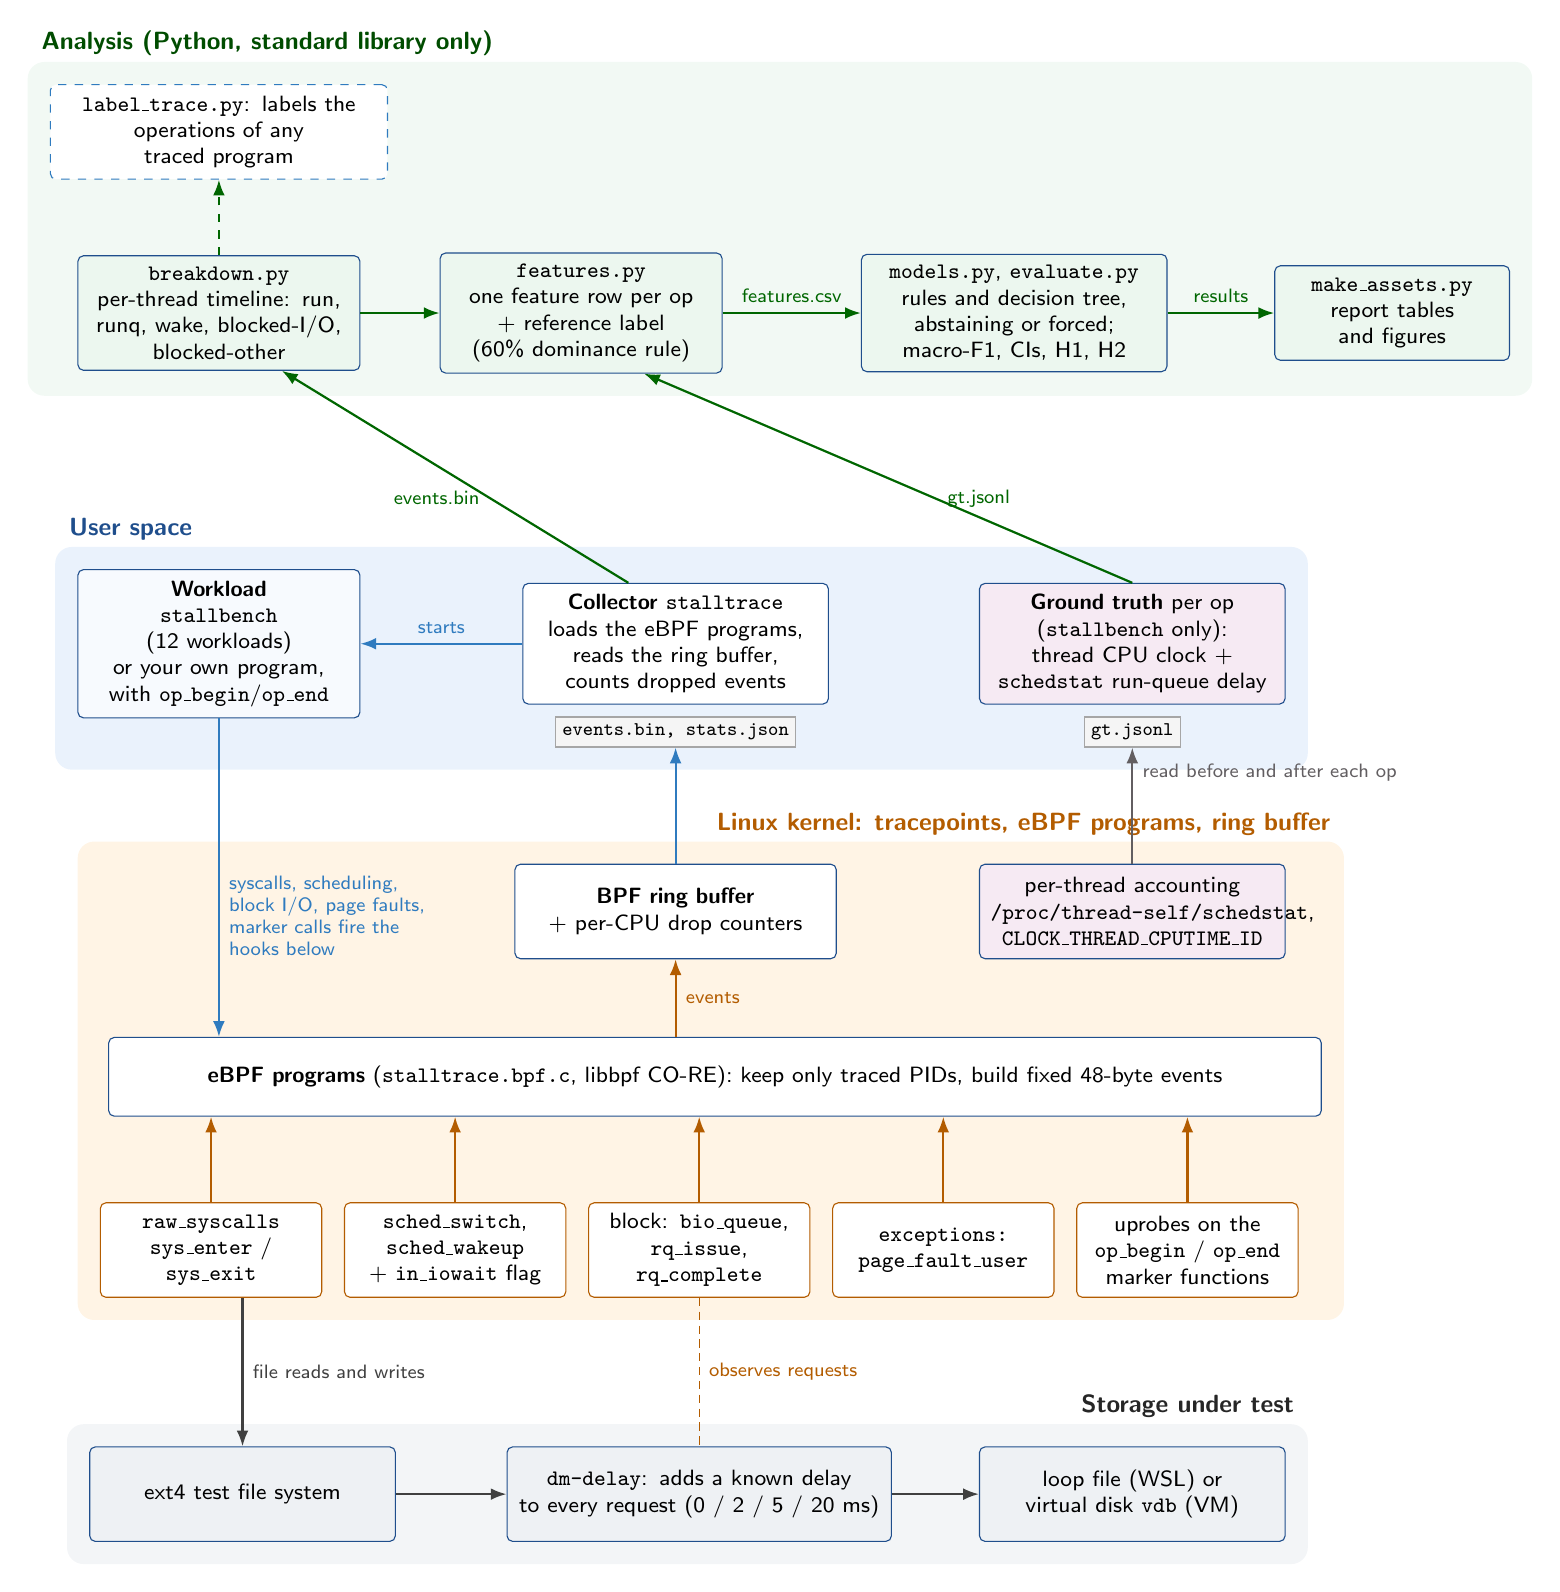
\begin{tikzpicture}[font=\footnotesize, >={Latex[length=2mm]},
  box/.style={draw=acc, rounded corners=2pt, fill=white, align=center, inner sep=4pt, minimum height=12mm},
  hook/.style={draw=kh, rounded corners=2pt, fill=white, align=center, inner sep=3pt,
               minimum height=12mm, text width=26mm},
  file/.style={draw=gray!70, fill=gray!8, align=center, inner sep=2.5pt, font=\scriptsize\ttfamily},
  arr/.style={->, thick, acc2},
  data/.style={->, thick, green!40!black},
  up/.style={->, thick, kh},
  lane/.style={rounded corners=6pt, inner sep=8pt},
  lbl/.style={font=\bfseries\small, anchor=south west, inner sep=1pt},
  note/.style={font=\scriptsize, align=center}]

% ================= analysis (top)
\node[box, text width=40mm, dashed, draw=acc2] (lt) at (1.6, 2.3) {\texttt{label\_trace.py}: labels the\\operations of any traced program};
\node[box, text width=33mm, fill=ana] (bd) at (1.6, 0) {\texttt{breakdown.py}\\per-thread timeline: run,\\runq, wake, blocked-I/O,\\blocked-other};
\node[box, text width=33mm, fill=ana] (ft) at (6.2, 0) {\texttt{features.py}\\one feature row per op\\+ reference label\\(60\% dominance rule)};
\node[box, text width=36mm, fill=ana] (ev) at (11.7, 0) {\texttt{models.py}, \texttt{evaluate.py}\\rules and decision tree,\\abstaining or forced;\\macro-F1, CIs, H1, H2};
\node[box, text width=27mm, fill=ana] (rep) at (16.5, 0) {\texttt{make\_assets.py}\\report tables\\and figures};

% ================= user space
\node[box, text width=33mm, fill=usr!40] (wl) at (1.6, -4.2) {\textbf{Workload}\\\texttt{stallbench} (12 workloads)\\or your own program,\\with \texttt{op\_begin}/\texttt{op\_end}};
\node[box, text width=36mm] (col) at (7.4, -4.2) {\textbf{Collector} \texttt{stalltrace}\\loads the eBPF programs,\\reads the ring buffer,\\counts dropped events};
\node[box, text width=36mm, fill=gtc] (gt) at (13.2, -4.2) {\textbf{Ground truth} per op\\(\texttt{stallbench} only):\\thread CPU clock +\\\texttt{schedstat} run-queue delay};

% ================= kernel
\node[box, text width=38mm] (rb) at (7.4, -7.6) {\textbf{BPF ring buffer}\\+ per-CPU drop counters};
\node[box, text width=36mm, fill=gtc] (acct) at (13.2, -7.6) {per-thread accounting\\\texttt{/proc/thread-self/schedstat},\\\texttt{CLOCK\_THREAD\_CPUTIME\_ID}};
\node[box, minimum width=154mm, minimum height=10mm] (prog) at (7.9, -9.7)
  {\textbf{eBPF programs} (\texttt{stalltrace.bpf.c}, libbpf CO-RE): keep only traced PIDs, build fixed 48-byte events};
\node[hook] (sys) at (1.5, -11.9) {\texttt{raw\_syscalls}\\\texttt{sys\_enter} / \texttt{sys\_exit}};
\node[hook] (sch) at (4.6, -11.9) {\texttt{sched\_switch},\\\texttt{sched\_wakeup}\\+ \texttt{in\_iowait} flag};
\node[hook] (blk) at (7.7, -11.9) {block: \texttt{bio\_queue},\\\texttt{rq\_issue},\\\texttt{rq\_complete}};
\node[hook] (pf) at (10.8, -11.9) {\texttt{exceptions:}\\\texttt{page\_fault\_user}};
\node[hook] (upr) at (13.9, -11.9) {uprobes on the\\\texttt{op\_begin} / \texttt{op\_end}\\marker functions};

% ================= storage
\node[box, text width=36mm, fill=sto] (fs) at (1.9, -15.0) {ext4 test file system};
\node[box, text width=46mm, fill=sto] (dm) at (7.7, -15.0) {\textbf{\texttt{dm-delay}}: adds a known delay\\to every request (0 / 2 / 5 / 20 ms)};
\node[box, text width=36mm, fill=sto] (disk) at (13.2, -15.0) {loop file (WSL) or\\virtual disk \texttt{vdb} (VM)};

% output files
\node[file, anchor=north] (f1) at ($(col.south)+(0,-1.5mm)$) {events.bin, stats.json};
\node[file, anchor=north] (f2) at ($(gt.south)+(0,-1.5mm)$) {gt.jsonl};

% ================= lanes
\begin{scope}[on background layer]
  \node[lane, fill=ana!70, fit=(lt)(bd)(ft)(ev)(rep)] (Lana) {};
  \node[lane, fill=usr, fit=(wl)(col)(gt)(f1)(f2)] (Lusr) {};
  \node[lane, fill=krn, fit=(rb)(acct)(prog)(sys)(upr)] (Lkrn) {};
  \node[lane, fill=sto!70, fit=(fs)(dm)(disk)] (Lsto) {};
\end{scope}
\node[lbl, text=green!30!black] at ($(Lana.north west)+(4pt,1pt)$) {Analysis (Python, standard library only)};
\node[lbl, text=acc] at ($(Lusr.north west)+(4pt,1pt)$) {User space};
\node[lbl, text=kh, anchor=south east] at ($(Lkrn.north east)+(-4pt,1pt)$) {Linux kernel: tracepoints, eBPF programs, ring buffer};
\node[lbl, text=gray!30!black, anchor=south east] at ($(Lsto.north east)+(-4pt,1pt)$) {Storage under test};

% ================= arrows
% kernel: hooks fire -> programs -> ring buffer -> collector
\foreach \h in {sys,sch,blk,pf,upr} \draw[up] (\h.north) -- (\h.north |- prog.south);
\draw[up] (prog.north -| rb.south) -- node[right, note] {events} (rb.south);
\draw[arr] (rb.north) -- (f1.south);
\draw[arr, gtc!40!black] (acct.north) -- node[right, note, pos=.78] {read before and after each op} (f2.south);
% workload -> kernel and storage
\draw[arr] (wl.south) -- node[right, note, pos=.62, align=left] {syscalls, scheduling,\\block I/O, page faults,\\marker calls fire the\\hooks below} (wl.south |- prog.north);
\draw[arr] (col.west) -- node[above, note] {starts} (wl.east);
\draw[->, thick, gray!50!black] (sys.south -| fs.north) -- node[right, note] {file reads and writes} (fs.north);
\draw[->, thick, gray!50!black] (fs.east) -- (dm.west);
\draw[->, thick, gray!50!black] (dm.east) -- (disk.west);
\draw[densely dashed, kh] (blk.south) -- node[right, note] {observes requests} (blk.south |- dm.north);
% analysis
\draw[data] ($(col.north)+(-6mm,0)$) -- node[left, note, pos=.4] {events.bin} ($(bd.south)+(8mm,0)$);
\draw[data] (gt.north) -- node[right, note, pos=.4] {gt.jsonl} ($(ft.south)+(8mm,0)$);
\draw[data] (bd.east) -- (ft.west);
\draw[data] (ft.east) -- node[above, note] {features.csv} (ev.west);
\draw[data] (ev.east) -- node[above, note] {results} (rep.west);
\draw[data, dashed] (bd.north) -- (lt.south);
\end{tikzpicture}
\end{document}
